\subsection{Finger grasping model}
\begin{samepage}
    At last, we have also to model the \textbf{finger grasping} the device, we can derive the model from the one used in the paper \cite{Finger_grasping_model} for the human finger.
    \nopagebreak

    \begin{figure}[H]
        \centering
        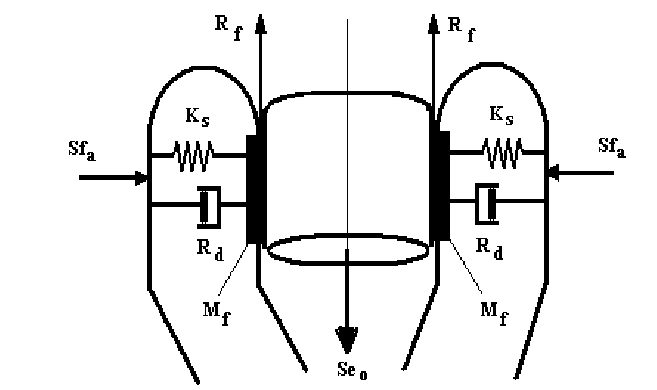
\includegraphics[width = 0.5\linewidth]{Chapters/Chapter2/Modelling_of_Entire_System/Figures/Model-of-two-soft-fingers-grasping-the-object.png}
        \caption{Model of two soft fingers grasping the object.}
        \label{fig: Finger_grasping_model}
    \end{figure}
\end{samepage}

This model describes two fingers grasping an object, for our case, we can simplify it to a \textbf{single finger grasping} the device.
Also, we can \textbf{neglect the friction} between the finger and the device as the device will be tested positioned on a flat surface with only the finger touching it from above.
\begin{figure}[H]
    \centering
    \resizebox{.7\linewidth}{!}{
        \begin{tikzpicture}
    \begin{scope}[every node/.style={bgelement}]
        \node (start) at (0,0) {};
        \node[right=1 of start] (w1) {1};
        \node[above=1 of w1] (Mf) {I: M\textsubscript{f}};
        \node[right=1 of w1] (v) {0};
        \node[above=1 of v] (w2) {1};
        \node[above=1 of w2] (Rdf) {R: Rd\textsubscript{f}};
        \node[right=1 of w2] (Cf) {C: $\frac{1}{Ks_{f}}$};
        \node[right=1 of v] (Sfa) {Sf\textsubscript{a}};
    \end{scope}
    \draw[bonds]
    (start) edge [e_out, flow={v}, effort={F}] (w1)
    (w1) edge [e_out] (Mf)
    (w1) edge [e_in] (v)
    (v) edge [e_in] (w2)
    (w2) edge [e_in] (Rdf)
    (w2) edge [e_in] (Cf)
    (Sfa) edge [e_out] (v);
\end{tikzpicture}
    }
    \caption{Bond graph of the finger grasping model.}
    \label{fig: Finger_grasping_bond_graph}
\end{figure}

The finger grasping can be modeled as a \textbf{mass-spring-damper} system, where the inertia component is represented by the finger's mass, while the spring and damper represent respectively the stiffness and damping effect of the finger's skin.

Human skin's properties have been studied by a team from the University École Centrale de Lyon, they found it has a stiffness constant ranging between \textbf{47.3 and 128.3 N/m}, and a damping coefficient between \textbf{0.08 and 0.121 Ns/m} \cite{Mech_characteristics_of_human_skin}.
The mass of the finger varies a lot depending on the finger's size.
